% Chapter 1

\chapter{Background and Literature Review} % Main chapter title

\label{Chapter2} % Change X to a consecutive number; for referencing this chapter elsewhere, use \ref{ChapterX}

\lhead{Chapter 2. \emph{Introduction}} % Change X to a consecutive number; this is for the header on each page - perhaps a shortened title

%----------------------------------------------------------------------------------------
%	SECTION 1
%----------------------------------------------------------------------------------------


\section{Artificial Neural Networks}
\subsection{ANN : a framework for many different machine learning algorithms}

Artificial neural networks have been conceptualized on the purpose to mimic how the human brain performs a task via the use of simplified mathematical models. A neural network is a machine learning algorithm as it is capable to learn, recognize patterns and generalize. 

Some machine learning implementations can deal with certain tasks more efficiently than human brain. For example, in chess, the program DeepBlue managed to beat the world champion Kasparov in 1997. 20 years after, for the game go, the program AlphaGo also managed to beat the best go player in the world. Nevertheless, computers are not able of equaling the brain's cognitive capacity, its flexibility, robustness and energy efficiency. Indeed, neural network are mono task, they can perform well for only precise task to answer one problem, brains can do several different tasks and also in the same time.

Machine learning has four learning paradigms, which correspond to a particular task.

The first one is called predictive or supervised learning. Its purpose is to learn a mapping function from a know data and its label. This function can then be reused to find the classification of new data. 

The second one is called descriptive or unsupervised learning. This type of learning is more complex and abstract to understand than supervised learning because the purpose is to group training data for which we don't know the labels into clusters by using a similarity metric. 
A cluster is a group of data which share similar elements.
The aim is to produce new knowledge by discovering hidden structure in the data.

The third type is semi-supervised learning. As indicated by its name this algorithm is a mix between the two other algorithms : most of the data is unlabelled, only a part is to identify the different groups which compose the set. This method is supposed to be more efficient that unsupervised learning without the time and costs needed to label all the data in supervised learning.

The last type of learning is reinforcement learning. Without annotated data like unsupervised learning, this type manages to find connections between data based on the use of rewards and punishments.

In this paper, all the neural networks mentioned use supervised learning.



\subsection{Single-layer perceptron}

In 1943, McCulloch and Pitts proposed the first conception of a formal neuron model \cite{mcculloch}. An artificial neuron is a biologically inspired mathematical model that mimics the basic functions of biological neurons: processes information and transmits it \cite{neuron}. 

Single layer perceptron is the most basic ANN. It is composed by an input and an output layer containing one neuron or more also called node. The input layer receives the data to be processed and the output layer makes the prediction about the input. Even if there are two layers, this architecture is called single layer perceptron as no computation is made in the input layer. The full process is divided into two times : first the forward propagation and then the backpropagation. 

During the forward propagation, the neuron in the output layer is fed by inputs data which are, for example, pixels from an image. Every pixel is associated to a weight which is randomly initialized. 
The first step of the process made by this neuron is to sum all these pixels values with their weights into a variable $Z$.

\begin{equation}
Z=w^T x + b
\end{equation}
where:

$w^T$ is the transpose of the weight matrix 

$x$ is the matrix containing the values of the pixels of the input  

$b$  the bias 

The bias shifts the decision boundary and does not depend on any input value, it is often initialized at 0.

Then, this function is submitted to an activation function that fire when the out of this function is above a threshold.

\begin{figure}[htbp]
  \centering
    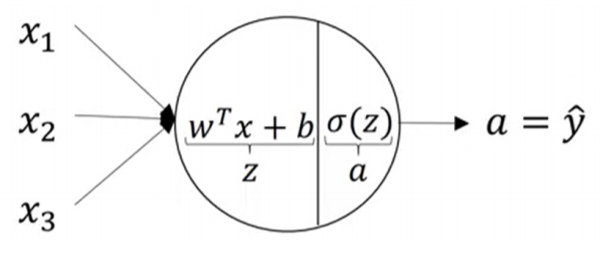
\includegraphics[width=\textwidth]{Figures/Perceptron.png}
    \rule{35em}{0.5pt}
  \caption[Schema of a perceptron]{Schema of a perceptron}
  \label{fig:Perceptron}
\end{figure}


During the backpropagation, the gradient descent algorithm is applied. The aim of the classification process is to minimize the cost. The cost is the average of all the losses which represent the errors between the predictions of the model and the real labels of the pictures. To minimize this cost, we can transform the training task of the ANN into an optimization problem by using a gradient descent, which is a local search algorithm. This algorithm is be used to find the local minimum for a differentiable function. This local minimum corresponds to the state where the model has the best accuracy. Thereby, the process goes backward in the network to update the weights and the bias to decrease the cost and so the number of errors by applying learning rules. 

This algorithm is repeated until the cost has converged.

Let's suppose we want to recognize if a picture contains a cat (label 1) or not (label 0), we can use in the output layer, the activation function sigmoid which returns a value between 0 and 1.

\begin{equation}
{\hat{y}} = {sigmoid(Z)}=\frac{1}{1+e^{-Z} }
\end{equation}
where:

$\hat{y}$ is the label prediction made by the neuron

The predicted label is then set as 1 if the output of the function \emph{sigmoid} is above a treshold, for example 0,5. There are a lot of different activation functions and they are chosen regarding the nature of the task. 




\subsection{Multi-layer perceptron}

Like the previous architecture, multi-layer perceptron is composed by an input and an output layer and also one or several hidden layers. Each hidden layer contains a specific number of nodes. In this architecture, each node is connected to every node in the adjacent layers but not to the nodes in the same layer. This type of connections where the data flow in one direction is called feedforward, there is no recursivity. 

During the forward propagation, the hidden layers apply activation functions on their inputs and transmit the information between the input and the output layer.



\begin{figure}[H]
  \centering
    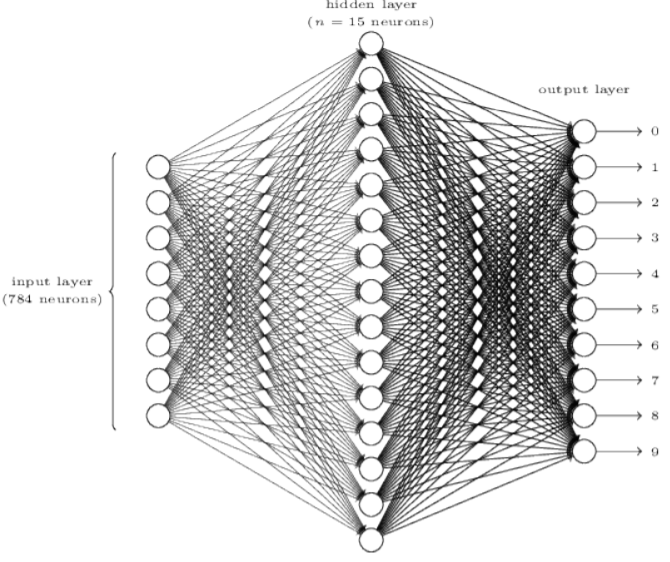
\includegraphics[width=\textwidth]{Figures/multi_layer.png}
    \rule{35em}{0.5pt}
  \caption[Schema of a multi-layer perceptron]{Schema of a multi-layer perceptron with one hidden layer composed by 15 neurons for a classification task involving 10 differents classes}
  \label{fig:Muli-layer perceptron}
\end{figure}

The reason to use this kind of architecture is that it has been demonstrated standard multi-layer feedforward networks with as few as a single hidden layer and arbitrary bounded and nonconstant activation function can approximate any continuous function \cite{multi}.
Indeed, ANN without hidden units can only produce limited mapping model. During the backpropagation, the learning rules are both applied in the hidden layer(s) and in the output layer and this makes the model performing better for more complex classification tasks.

Let's suppose we want to classify pictures into 10 classes. We can use a multi-layer perceptron which output layer is composed by 10 neurons. The activation function sigmoid can be used for the nodes in the hidden layer but not in the output one. We have to use the softmax activation function which is the corresponding function of sigmoid activation for more than two classes. It assigns decimal probabilities to each class. The sum of these decimals must be 1.0. 

\begin{equation}
{softmax(x)_{j}}=\frac{e^{{Z}_{j}}}{\sum_{i=1}^k e^{Z_{i}} }
\end{equation}

where:

${x}$ is the input picture

${j}$ is any particular class we want to get the probability

${k}$ is the number of classes

${Z}$ is the variable that sum all the input values with their associated weights (see equation 2.1) 

To get the prediction of the model for an input, we simply need to recover the corresponding class to the highest probability returned by \emph{softmax}.

 

\section{Convolutional neural networks}
\subsection{Overview}
Machine learning algorithms are good to process a small amount of data but they don't scale well for a large amount. This is the main reason which explain the elaboration of deep neural networks. A lot of different libraries (Theano, TensorFlow, Torch) and interfaces (Keras,Lasagne,Blocks) have been created in order to make their implementations easier without a deep understanding of the maths theory, high-level programming skills and potential code issues. 

Convolutional neural network is one of the most famous deep neural network which is directly inspired by the primary visual cortex of the brain \cite{CNN}.  

It is a type of feedforward neural network made up of neurons that have learnable weights and biases, very similar to the multi-layer perceptron.

CNNs are designed to process different data types but they are mainly used to classify two dimensional images. 


\subsection {AlexNet}
\subsection {VGGNet}
\subsection {GoogLeNet}
\section{Robustness of neural netwoks}



\section{Methods to find adversarial examples}

Different methods have been studied to improve robustness of neural networks \cite{survey}. 
These methods are used to provide guarantee on the safety of networks. Basically an adversarial example can be found by adding to an image natural perturbations such as fog or sunlight. Despite these perturbations, humans will not misclassify the image.

There are three main types of studies concerning adversarial attacks:

- The first one is about non-targeted adversarial attacks. This method consists of modifying the original image to make the network classify it at another random class.

- The second subject area deals with targeted adversarial attacks. This method targets, as its name assumes, one type of class to misclassify it into another precise one.

- The third study concerns defenses against adversarial attacks. This field deals with the problematic of building robust classifiers which are not fooled by adversarial examples. 

Famous methods to find adversarial examples :

- fast gradient sign FGSM

This method is the root of many other methods. The main idea of this method is to add noise to an image at each step of the process to classify an image. Adversarial examples can be easily found on models which use linearity. FSM is based on this assumption and uses the sign or the gradient of the loss function of the model to add or subtract small error to each pixel

- Projected Gradient Descent

This method is a multi-step variant of FGSM and it is why it's more efficient than it. Indeed FGSM is a one-step approach.
It works well for high dimensions cases. 
If a network resist to attacks made with this method, it means it is robust against a lot of other attacks.


- Basic Iterative Method (IBM)

This method is an iterative version of FGSM. This method is more efficient than FGSM because the noise is applied many times instead of once.  Networks which are trained to be robust against one-step adversarial attacks should fail with the attacks made with this method. To avoid put to much noise, the pixel are clipped.


- Carlini-Wagner

This method is able to find each time an adversarial example on defensively distilled and undistilled networks by proposing  3 attacks from 3  different algorithms L0 L2 Linf.  Defensive distillation is a method used to improve the robustness of a network against adversarial examples.

L0 attack  is the first one which manage to find adversarial example one images from the database ImageNet


-Jacobian-based Saliency Map Approach (JSMA)

FSMA is a method  used for targeted misclassification and looks for the smallest perturbation to fool the classification. Compared to the other methods that use output variations to find the related input changes, JSMA builds a map between the input modifications and the output variations. This method is called forward derivative. Like IBM, this method iteratively perturbs features of input data which are the most likely to lead a misclassification with constant offset until the target misclassification is found.

 














%----------------------------------------------------------------------------------------
%	SECTION 2
%----------------------------------------------------------------------------------------

\section{Methods used in Research Papers to evaluate robustness of the neural netwoks}
\subsection {DLV}
\subsection {Two-player game}
\subsection {DeepPoly}

